\themaM
\graphicspath{{../Ch8_Longueurs_et_perimetre/Images/}}

\chapter{Périmètres\\et formules}
\label{C16}


%%%%%%%%%%%%%%%%%%%%%%%%%%%%%%%%%%%%%%%%%%
\begin{prerequis}[Connaissances et compétences abordées]
   \begin{itemize}
      \item Calculer le périmètre d’un carré et d’un rectangle, la longueur d’un cercle, en utilisant une formule.
   \end{itemize}
\end{prerequis}

\vfill

\begin{debat}[Débat : ce fabuleux nombre $\pi$] 
   $\pi$ est un nombre, au même titre que 2 ou 100, ou 6,538. Il désigne le rapport du périmètre d'un cercle par son diamètre. Il a fasciné de nombreux savants depuis l'antiquité et il existe des livres entiers qui lui sont consacrés !
   \begin{center}
      \DeclareFixedFont{\ps}{U}{psy}{m}{n}{7cm}
      \begin{pspicture}(-3,-3)(3,3)
         \rput(0,-2){\pscharpath[linecolor=B2,fillstyle=solid,fillcolor=B2,opacity=0.5]{\rput[b](0,0){\ps p}}}
         \pstextpath{
            \pscustom[linestyle=none]{%
               \parametricplot[plotpoints=500]{0}{1350}{t cos t 500 div mul t sin t 500 div mul}
               \psline(!51 cos 51 600 div mul 600 add 51 sin 3510 600 div mul)}}
               {3,141 592 653 589 793 238 462 643 383 279 502 884 197 169 399 375 105 820 974 944 592 307 816 406 286 208 998 628 034 825 342 117 067 982 148 086 513 282 306 647 093 844 609 550 582 231 725 359 408 128 481 117 450 284 102 701 938 521 105 559 644 622 948 954 930\dots}
      \end{pspicture}
   \end{center}
   \bigskip
   \begin{cadre}[B2][F4]
      \begin{center}
         Vidéos : \href{https://leblob.fr/fondamental/le-nombre-pi}{\bf Le nombre Pi}, site Internet {\it Le Blob}, épisode des {\it Petits contes mathématiques}. \\
         \href{https://www.mypiday.com/}{Un site pour trouver sa date de naissance dans les décimales de $\pi$.}
      \end{center}
   \end{cadre}
\end{debat}

\vfill

\textcolor{PartieGeometrie}{\sffamily\bfseries Cahier de compétences} : chapitre 11, exercices 2 ; 5 ; 7 à 11 ; 38 ; 39.


%%%%%%%%%%%%%%%%%%%%%%%%%%%%%%%%%%%%
%%%%%%%%%%%%%%%%%%%%%%%%%%%%%%%%%%%%
\activites

\begin{activite}[À la découverte du nombre $\pi$]
   {\bf Objectifs :} retrouver la formule donnant la longueur d’un cercle ; traiter un problème de proportionnalité ; organiser des données.
   \begin{QCM}
      Par groupe de trois ou quatre, choisir cinq objets circulaires parmi ceux    disponibles dans la classe.
      \begin{center}
         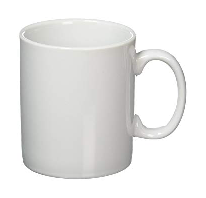
\includegraphics[height=2cm]{tasse}
         \qquad
         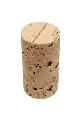
\includegraphics[height=2cm]{bouchon}
         \qquad
         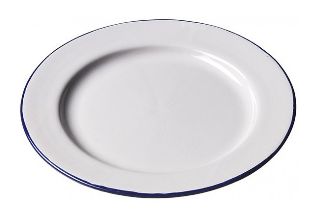
\includegraphics[height=2cm]{assiette}
         \qquad
         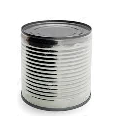
\includegraphics[height=2cm]{boite}
         \qquad
         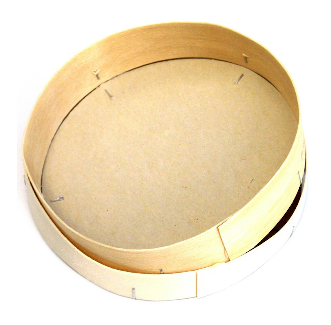
\includegraphics[height=2cm]{camembert}
      \end{center}
      \begin{minipage}{8cm}
         Pour chaque objet, il s'agit de mesurer le périmètre, c'est-à-dire la mesure de son contour à un endroit où l'objet est circulaire ; de mesurer son diamètre, et enfin d'effectuer le rapport de ces deux mesures.
      \end{minipage}
      \qquad
      \begin{minipage}{8cm}
         {\psset{yunit=0.4}
         \begin{pspicture}(-1.5,-1.5)(6,6.7)       
            \psline(4,1)(4,5)
            \psline(0,1)(0,5)
            \psellipse(2,5)(2,1)
            \psellipticarc(2,1)(2,1){180}{0}
            \psline[linewidth=1mm,linecolor=A1]{<->}(0,5)(4,5)
            \rput(5,5){\textcolor{A1}{diamètre}}
            \psellipticarc[linewidth=0.8mm,linecolor=B1](2,2.5)(2,1){188}{0}
            \psellipticarc[linewidth=0.8mm,linestyle=dashed,linecolor=B1]{->}(2,2.5)(2,1){0}{178}
            \rput(5,2.5){\textcolor{B1}{périmètre}}
         \end{pspicture}}
      \end{minipage}
      Pour cela, on dispose de différents outils et instruments de mesure : quel est le nom de chacun de ces instruments ?
      \begin{center}
         \begin{pspicture}(0,1.7)(16,8)
            \rput(5.5,7){
\includegraphics[width=9cm]{regle}}
            \rput(13.5,7){\hdashrule{4.5cm}{0.15pt}{4pt 2pt}}
            \rput(3,4.2){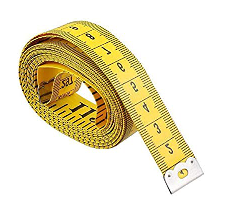
\includegraphics[width=3.5cm]{couturiere}}
            \rput(2.5,1.8){\hdashrule{4.5cm}{0.15pt}{4pt 2pt}}
            \rput(8,4.2){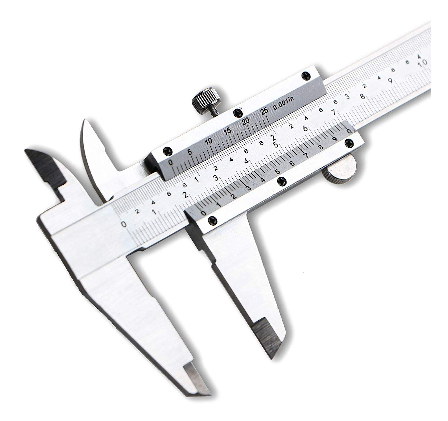
\includegraphics[width=3.5cm]{pied_coulisse}}
            \rput(8,1.8){\hdashrule{4.5cm}{0.15pt}{4pt 2pt}}
            \rput(13.5,4.2){
\includegraphics[width=4cm]{bande}}
            \rput(13.5,1.8){\hdashrule{4.5cm}{0.15pt}{4pt 2pt}}
         \end{pspicture}
      \end{center}
      Remplir le tableau suivant où $p\div d$ est le rapport entre le périmètre de l'objet et son diamètre.
      \begin{center}
         {\hautab{1.5}
         \begin{tabular}{|p{1.8cm}|*{5}{C{2.2}|}}
            \hline
            Objet & & & & & \\
            \hline
            Instrument & & & & & \\
            \hline
            Périmètre $p$ & & & & & \\
            \hline
            Diamètre $d$ & & & & & \\
            \hline
            $p\div d$ & & & & & \\
            \hline
         \end{tabular}}
      \end{center} \bigskip
      Que constate-t-on ? \pf \\
   \end{QCM}
\end{activite}


%%%%%%%%%%%%%%%%%%%%%%%%%%%%%%%%%%%
%%%%%%%%%%%%%%%%%%%%%%%%%%%%%%%%%%%
\cours 

%%%%%%%%%%%%%%%%%%%%%%%%
\section{Formules pour les polygones}

Le périmètre d'un polygone est la somme des longueurs de ses segments, on peut également utiliser des formules. \medskip

\begin{Ltableau}{0.97\linewidth}{4}{C{4}|p{2.6cm}|C{3.5}|p{4.5cm}}
   \hline 
   Figure plane & Formule & Exemple & Calcul \\
   \hline
   {\psset{unit=0.7}
   \begin{pspicture}(0,-0.5)(4,3.5) % carré
      \pstGeonode[PointName=none,linecolor=red,PointSymbol=none](0.5,0.5){A}(3.5,0.5){B}(3.5,3.5){C}(0.5,3.5){D}
      \psset{linecolor=A1}
      \pstSegmentMark{A}{B}
      \pstSegmentMark{B}{C}
      \pstSegmentMark{C}{D}
      \pstSegmentMark{D}{A}
      \rput(2,2){carré}
      \rput(2,0.1){\textcolor{A1}{$c$}}
      \rput(2,3.9){\textcolor{A1}{$c$}}
      \rput(0.1,2){\textcolor{A1}{$c$}}
      \rput(3.9,2){\textcolor{A1}{$c$}}
   \end{pspicture}}
   &
   \begin{minipage}[b]{3cm}
      $p =c+c+c+c$ \\ 
      $p =4\times c$ \\
      $p =4\,c$ \\ [8mm]
   \end{minipage}
   &
   \begin{pspicture}(0.3,0.2)(4,4)
      \psframe(1,1)(3,3)
      \psset{linestyle=dashed}
      \small
      \psline{<->}(1,0.7)(3,0.7)
      \rput(2,0.4){2 cm}
      \psline{<->}(0.7,1)(0.7,3)
      \rput{90}(0.4,2){2 cm}
      \psline{<->}(1,3.3)(3,3.3)
      \rput(2,3.6){2 cm}
      \psline{<->}(3.3,1)(3.3,3)
      \rput{90}(3.6,2){2 cm}
   \end{pspicture}
   &
   \begin{minipage}[b]{5cm}
      $p =\ucm{2}+\ucm{2}+\ucm{2}+\ucm{2}$ \\ 
      $p =4\times \ucm{2}$ \\
      $p =\ucm{8}$ \\ [8mm]
   \end{minipage} \\
   \hline
   \begin{pspicture}(0,.3)(4,3.5) % rectangle
      \pstGeonode[PointName=none,linecolor=B2,PointSymbol=none](0.5,1){A}(3.5,1){B}(3.5,3){C}(0.5,3){D}
      \pstSegmentMark[linecolor=B2]{A}{B}
      \pstSegmentMark[SegmentSymbol=MarkCros,linecolor=A1]{B}{C}
      \pstSegmentMark[linecolor=B2]{C}{D}
      \pstSegmentMark[SegmentSymbol=MarkCros,linecolor=A1]{D}{A}
      \rput(2,2){\small rectangle}
      \rput(2,0.6){\textcolor{B2}{$L$}}
      \rput(2,3.5){\textcolor{B2}{$L$}}
      \rput(0.1,2){\textcolor{A1}{$\ell$}}
      \rput(3.8,2){\textcolor{A1}{$\ell$}}
   \end{pspicture}
   &
   \begin{minipage}[b]{3cm}
      $p =L+\ell+L+\ell$ \\ 
      $p =2\times L+2\times\ell$ \\
      $p =2\times(L+\ell)$ \\
      $p =2\,(L+\ell)$ \\ [4mm]
   \end{minipage}
   &
   \begin{pspicture}(-0.2,-0.3)(3.5,3.3)
      {\psset{unit=0.8}
      \small
      \psframe(1,0.5)(3,3.5)
      \psline[linestyle=dashed]{<->}(1,0.2)(3,0.2)
      \rput(2,-0.1){\udm{0,2}}
      \psline[linestyle=dashed]{<->}(0.7,0.5)(0.7,3.5)
      \rput{90}(0.4,2){\udm{0,3}}}
   \end{pspicture}
   &
   \begin{minipage}[b]{5cm}
      $p =\udm{0,2}+\udm{0,3}+\udm{0,2}$ \\
      \hspace*{30mm} $+\udm{0,3}$ \\
      $p =2\times(\udm{0,2}+\udm{0,3})$ \\
      $p =2\times\udm{0,5}$ \\
      $p = \udm{1}$ \\
   \end{minipage} \\
   \hline
   {\psset{unit=0.9}
   \begin{pspicture}(0,0)(4,4) %triangle
      \pstGeonode[PointName=none,PointSymbol=none](0.5,0.5){A}(3.5,0.5){B}(1,3.5){C}
      \pstLineAB[linecolor=A1]{A}{B}
      \pstLineAB[linecolor=B1]{C}{B}
      \pstLineAB[linecolor=J1]{A}{C}
      \rput(1.7,1.4){triangle}
      \rput(2,0.1){\textcolor{A1}{$a$}}
      \rput(2.6,2.1){\textcolor{B1}{$b$}}
      \rput(0.4,1.9){\textcolor{J1}{$c$}}
   \end{pspicture}}
   &
   \begin{minipage}[b]{3cm}
      $p =a+b+c$ \\ [11mm]
   \end{minipage}
   &
   {\psset{unit=0.8}
   \small
   \begin{pspicture}(0,-0.3)(4,3)
      \pspolygon(0.5,0.7)(3.2,0.7)(3.2,3.5)
      \psline[linestyle=dashed]{<->}(0.5,0.4)(3.2,0.4)
      \rput(2,0.1){2,7 m}
      \psline[linestyle=dashed]{<->}(3.5,0.7)(3.5,3.5)
      \rput{90}(3.8,2){2,8 m}
      \psline[linestyle=dashed]{<->}(0.3,0.9)(3,3.7)
      \rput{45}(1.4,2.5){3,9 m}
   \end{pspicture}}
   &
   \begin{minipage}[b]{5cm}
      $p =\um{2,7}+\um{2,8}+\um{3,9}$ \\ 
      $p =\um{9,4}$ \\ [8mm]
   \end{minipage} \\
   \hline
\end{Ltableau}


%%%%%%%%%%%%%%%%%%%%%%%%%%%%%%%
\section{Circonférence d'un cercle}

Le cercle n'est pas un polygone, on ne peut donc pas calculer son périmètre de la même manière, il est alors indispensable d'utiliser une formule. \medskip

\begin{Ltableau}{0.97\linewidth}{4}{C{4}|p{2.6cm}|C{3.5}|p{4.5cm}}
   \hline 
   Figure plane & Formule & Exemple & Calcul \\
   \hline
   \begin{pspicture}(0,0.3)(4,3.7) %cercle
      \pscircle(2,2){1.3}
      \psdots(2,2)
      \psline[linecolor=A1,arrowsize=0.2]{<->}(2,2)(3.3,2)
      \rput(2.75,2.2){\textcolor{A1}{$r$}}
      \rput(2,1.6){cercle}
   \end{pspicture}
   &
   \begin{minipage}[b]{3cm}
      $p =2\times\pi\times r$ \\ 
      $p =2\,\pi\,r$ \\ [8mm]
   \end{minipage}
   &
   \begin{pspicture}(0.2,0.3)(4,3.7)
      \pscircle(2,2){1.3}
      \psline[linestyle=dashed,arrowsize=0.2]{<->}(2,2)(3.3,2)
      \rput(2.65,2.35){\ukm{1,2}}
   \end{pspicture}
   &
   \begin{minipage}[b]{5cm}
      $p =2\times\pi\times \ukm{1,2}$ \\ 
      $p \approx2\times3,14\times\ukm{1,2}$ \\
      $p \approx\ukm{7,54}$ \\ [8mm]
   \end{minipage} \\
   \hline
\end{Ltableau}

\begin{remarques}
   le périmètre d'un cercle de rayon $r$ est proportionnel à son diamètre (et donc à son rayon), il vaut $p =2\times\pi\times r$ où $\pi \simeq 3,141\,592\,653\,589\,793\,238\,462\,643\,383\,279\,50\dots$ \\
   Souvent, on choisit 3,14 comme valeur approchée ou on utilise la touche \fbox{$\pi$} de la calculatrice.
\end{remarques}


%%%%%%%%%%%%%%%%%%%%%%%%%%%%%%%%%%%
%%%%%%%%%%%%%%%%%%%%%%%%%%%%%%%%%%%
\exercicesbase

\begin{colonne*exercice}

\serie{Périmètre de polygones} %%%

\begin{exercice} %1
   Calculer le périmètre des figures suivantes. \\ [1mm]
   {\psset{unit=0.5}
   \small
   \begin{pspicture}(-3,-0.5)(5,4)
      \psframe(0,0)(4,3)
      \psframe(0,0)(0.3,0.3)
      \rput(2,0){x}
      \rput(2,3){x}
      \rput(0,1.5){=}
      \rput(4,1.5){=}
      \rput(2,-0.5){\um{6}}
      \rput{90}(-0.5,1.5){\um{4}}
   \end{pspicture}
   \begin{pspicture}(-1,0)(4,4.5)
      \psframe(0,0)(4,4)
      \psframe(0,0)(0.3,0.3)
      \rput(2,0){x}
      \rput(2,4){x}
      \rput(0,2){x}
      \rput(4,2){x}
      \rput(2,-0.5){\ucm{27}}
   \end{pspicture}
   
   \begin{pspicture}(-1,0)(4,6)
      \pspolygon(1,1)(7,1)(2,5)
      \psline(2,1)(2,5)
      \psframe(2,1)(2.3,1.3)
      \rput{-40}(5,3.3){\ucm{6,9}}
      \rput{78}(1,3){\ucm{4,6}}
      \rput(3.5,0.5){\ucm{6,6}}
      \rput{90}(2.5,2.7){\ucm{4,4}}
   \end{pspicture}
   \begin{pspicture}(4,1)(14,6)
      \pspolygon(8,2)(14,2)(8,5)
      \rput(11,1.5){\umm{83}}
      \rput{90}(7.5,3.5){\umm{25}}
      \rput{-30}(11,4){\umm{86,68}}
      \psframe(8,2)(8.3,2.3)
   \end{pspicture}}
\end{exercice}


\begin{exercice} %2
   Compléter le tableau suivant où $c$ est la longueur du côté du carré et $\mathcal{P}$ son périmètre.
   \begin{center}
      {\hautab{1.3}
      \begin{Ctableau}{0.9\linewidth}{5}{c}
         \hline
         $c$ & \ucm{3} & \udm{7} & & \\
         \hline
         $\mathcal{P}$ & & & \umm{32} & \ukm{15} \\
         \hline  
      \end{Ctableau}} \medskip
   \end{center}
\end{exercice}


\begin{exercice} %3
   Compléter le tableau suivant où $L$ est la longueur du côté du rectangle, $\ell$ sa largeur et $\mathcal{P}$ son périmètre.
   \begin{center}
      {\hautab{1.3}
      \begin{Ctableau}{0.9\linewidth}{5}{c}
         \hline
         $L$ &\udm{ 3,5} & \umm{7,4} & & \um{7,2} \\
         \hline
         $\ell$ & \udm{2,8} & \umm{21} & \ukm{3,75} & \\
         \hline
         $\mathcal{P}$ & & & \ukm{23} & \um{45} \\
         \hline  
      \end{Ctableau}}
   \end{center}
\end{exercice}

\medskip

\serie{Périmètre de cercles} %%%%%%%%%%%%%%%%

\begin{exercice} %4
   Calculer le périmètre des figures suivantes. \\
   {\psset{unit=0.5}
   \small
    \begin{pspicture}(-1.5,0)(6,6)
      \pscircle(3,3){2}
      \psline(3,3)(5,3)
      \rput(4,2.5){15 km}
   \end{pspicture}
   \begin{pspicture}(9.5,0)(14,6)
      \pscircle(12,3){2}
      \psline(10,3)(14,3)
      \rput(12,3.5){5,6 m}
   \end{pspicture}
   
   \begin{pspicture}(7,0.5)(14,6)
      \psarc(11,2){3}{0}{180}
      \psline(8,2)(14,2)
      \rput(11,1.5){\umm{8,3}}
   \end{pspicture}
   \begin{pspicture}(-2.5,0)(4,6.5)
      \psframe(0,0)(4,4)
      \psarc(2,4){2}{0}{180}
      \rput(2,4.6){\ucm{20}}
      \psdots(0,2)(2,4)(2,0)(4,2)
   \end{pspicture}
   }
\end{exercice}


\serie{Problèmes} %%%%%%%%%%%%%%%%%%

\begin{exercice} %5
   On considère la figure suivante :
   \begin{center}
   {\small
   \psset{unit=0.8}
      \begin{pspicture}(0,-0.7)(5,2.5)
         \pspolygon(0,0)(5,0)(2,2)(0,2)
         \psline[linestyle=dashed](2,2)(1.5,0)
         \psframe(0,0)(0.2,0.2)
         \psframe(0,2)(0.2,1.8)
         \rput(-0.3,-0.3){D}
         \rput(-0.3,2.3){A}
         \rput(5.3,0){C}
         \rput(2,2.3){B}
         \rput(1.5,-0.3){M}
         \rput(1,2.3){2 cm}
         \rput{90}(-0.3,1){\ucm{3}}
         \psline{<->}(0,-0.7)(5,-0.7)
         \rput(2.5,-1){\ucm{6}}
         \rput{-30}(4,1){\ucm{5}}
      \end{pspicture}}
   \end{center}
   \begin{enumerate}
      \item On suppose que DM$ =\ucm{1}$, comparer le périmètre du quadrilatère ABMD et celui du triangle BCM.
      \item Même question si DM$ =\ucm{5}$.
      \item Déterminer la position du point M pour que ces deux périmètres soient égaux.
   \end{enumerate}
\end{exercice}


\begin{exercice}
   On considère la figure suivante : \\
   {\psset{unit=0.5,linewidth=0.5mm}
   \small
   \begin{pspicture}(-3,-3)(10,3.5)
      \psgrid[subgriddiv=0,gridlabels=0pt,gridcolor=lightgray](0,-3)(10,3)
      \psarc(2,0){2}{180}{0}
      \psarc(3,0){3}{180}{0}
      \psarc(8,0){2}{0}{180}
      \psarc(7,0){3}{0}{180}
      \psline{<->}(8,-1)(9,-1)
      \rput(8.5,-1.5){\ucm{2}}
   \end{pspicture}}
   \begin{enumerate}
      \item De quoi est composée cette figure ?
      \item Déterminer alors son périmètre.
   \end{enumerate}
\end{exercice}

\begin{exercice}
   On considère la figure suivante : \\
   {\psset{unit=0.5,linewidth=0.5mm}
   \small
    \begin{pspicture}(-4,-1)(8,4.5)
      \psgrid[subgriddiv=0,gridlabels=0pt,gridcolor=lightgray](-1,-1)(8,4)
      \psarc(3,0){3}{90}{180}
      \psarc(3,1){2}{0}{90}
      \psarc(4,1){1}{-90}{0}
      \psline(0,0)(4,0)
      \psline{<->}(6,2)(7,2)
      \rput(6.5,1.5){\ucm{4}}
      \psset{linewidth=0.4mm}
      \psline(3,0)(3,3)
      \psline(3,1)(5,1)
      \psline(4,0)(4,1)
   \end{pspicture}}
   \begin{enumerate}
      \item De quoi est composée cette figure ?
      \item Déterminer alors son périmètre.
   \end{enumerate}
\end{exercice}

\medskip

\begin{exercice}
   Le couloir le plus à l'intérieur d'une piste d'athlétisme est composé de deux lignes droites de 100 mètres et de deux demi-cercles de rayon 31,83 mètres.
\begin{enumerate}
   \item On considère que la distance parcourue est celle correspondant à la ligne la plus intérieure de son couloir. Vérifier que la distance d’un tour de piste complet parcourue dans le couloir 1 est d’environ 400 m.
  \item Pourquoi y a-t-il un décalage des coureurs au départ d’une course de 400 m ?
\end{enumerate}
\end{exercice}

\end{colonne*exercice}


%%%%%%%%%%%%%%%%%%%%%%%%%%%%%%%%%%%%
\Recreation

\enigme[Quelques représentations de $\pi$]
   \partie[un moyen mnémotechnique pour apprendre $\pi$]
     Dans la plupart des cas, deux décimales de $\pi$ suffisent pour la majorité des calculs, c'est-à-dire 3,14. \\
     Pour retenir quelques-unes des autres décimales, il existe des moyens mnémotechniques donnant les chiffres de $\pi$ : il s'agit de remplacer chaque mot par le nombre de lettres qui le composent. \\
     Donner une valeur approchée de $\pi$ à partir de la phrase suivante : \og {\it May I have a large container of coffee ?} \fg \\ [2mm]
     \pf \\ [2mm]
     Même chose avec cette poésie : \og {\it Que j'aime à faire apprendre un nombre utile aux sages. Immortel Archimède, artiste, ingénieur ! Qui de ton jugement peut priser la valeur ? Pour moi, ton problème eut de pareils avantages.} \fg \\ [2mm]
      \pf \\ [2mm]
   
   \partie[les approximations]
      On ne pourra jamais connaître la valeur exacte de $\pi$ puisque c'est un nombre \og qui ne se termine pas \fg. Actuellement, on connait grâce à plusieurs très gros calculateurs près de 31\,000 milliards de chiffres à $\pi$ ! La course aux décimales de $\pi$ a commencé très tôt dans l'antiquité. \\
      Compléter le tableau suivant des valeurs approchées de $\pi$, puis donner le nombre de décimales exactes.
      \begin{center}
         {\hautab{2.2} 
         \small 
         \begin{Ltableau}{0.9\linewidth}{5}{c}%|C{1.5}|C{4.5}|C{4}|C{2}|C{2}|}
           \hline
            année approximative& pays & approximation & valeur approchée & décimales exactes \\
            \hline
            $- 2000$ & Babylone & $3+\dfrac{1}{8}$ & & \\
            \hline
            $- 1650$ & Egypte  & $\left(\dfrac{16}{9}\right)^2$ & & \\
            \hline
            $- 250$ & Grèce & $\dfrac{223}{71} < \pi < \dfrac{22}{7}$ & & \\
            \hline
            $640$ & Inde & $\sqrt{10}$ & & \\
            \hline
            $1464$ & Allemagne & $\dfrac34(\sqrt3+\sqrt6)$ & & \\
            \hline
         \end{Ltableau}} \bigskip
      \end{center}

   \partie[les formules]
      Avec le développement de techniques de calcul plus poussées, les mathématiciens écrivent des formules pour calculer $\pi$, voilà un florilège de quelques-unes de ces formules curieuses\dots \\
      \begin{itemize}
         \item Wallis en 1655 : \qquad $\pi = \displaystyle{2\prod_{n=1}^{\infty}\frac{4n^2}{4n^2-1}}$ \\ [1mm]
         \item Leibniz en 1674 : \quad $\pi =\displaystyle{8\sum_{k=0}^{\infty}\frac{1}{(4k+1)(4k+3)}}$ \\
         \item Euler en 1760 : \qquad $\pi =20\arctan\dfrac17+8\arctan\dfrac{3}{79}$
      \end{itemize}
  

  
   


